\documentclass[14pt,aspectratio=169]{beamer}

\usepackage[english, spanish]{babel}
% \usepackage[T1]{fontenc}
% \usepackage[utf8]{inputenc}
\usepackage{minted}
\usepackage[nodayofweek,level]{datetime}
\usepackage{hyperref}
\usepackage{url}
\usepackage{bibentry}
\usepackage{graphicx}
\usepackage{booktabs} % Allows the use of \toprule,
\usepackage{xcolor}
\usepackage{simplebnf}
\usepackage{multicol}
% \usepackage{biblatex}
% \addbibresource{biblo.bib}
\setlength{\columnsep}{0.2cm}

% %% Definiciones de comandos
\newcommand{\mydate}{\formatdate{29}{02}{2024}}
\graphicspath{ {images/} }
\beamertemplatenavigationsymbolsempty

%%%%%%%%%%%%%%%%%%%%%%%%%%%%%%%%%%%%%%%%%%%%%%%%%%%%%%%%%%%%%%%%%%%%%%%%
%% Tema y estilo de la presentación
\usetheme{Madrid}
\author[Miguel E. Ruiz]{Miguel E. Ruiz}
\title[\texttt{Madrid |> Elixir}]{Cómo conocí a la metaprogramación\\ (y sobreviví a ello)}
\date{\mydate}

%%%%%%%%%%%%%%%%%%%%%%%%%%%%%%%%%%%%%%%%%%%%%%%%%%%%%%%%%%%%%%%%%%%%%%%%
%% Empieza el documento

\begin{document}

\begin{frame}
  \titlepage
\end{frame}

\begin{frame}{Contenidos}
  \tableofcontents[hideallsubsections]
\end{frame}

\section{Introducción}
\begin{frame}{\texttt{IO.puts("Hello, World!")}}
  \begin{columns}
    \begin{column}{0.5\textwidth}
      \centering
      
\includegraphics[width=0.8\textwidth]{me-formal.jpg}
    \end{column}

    \begin{column}{0.5\textwidth}
      \begin{itemize}
        \item \texttt{Miguel [Emilio]}
        \item Ingeniero Informático
        \item Intereses: Programación funcional y concurrente
        \item Erlang y Elixir
      \end{itemize}
    \end{column}
  \end{columns}
\end{frame}

\begin{frame}{La metaprogramación y yo}
  \begin{itemize}
    \item Al acabar el Grado (2018), interés en Elixir
    \begin{itemize}
      \item Ejercicios en Codewars
      \item Proyecto Pokedex
    \end{itemize}
    \item Interés en el libro \textit{Metaprogramming Elixir}
    \item Sin embargo\dots
    \begin{itemize}
      \item Falta de tiempo (y de motivación)
    \end{itemize}
    \item Arranca el máster (2021) y\dots
    \begin{itemize}
      \item recupero el interés en la metaprogramación
      \item posibilidad de hacer el TFM sobre ello
    \end{itemize}
  \end{itemize}
\end{frame}

\begin{frame}{Una cosa os prometo...}
  \begin{columns}
    \begin{column}{0.5\textwidth}
      \centering
      
\includegraphics[width=0.8\textwidth]{charlie_day.png}
    \end{column}

    \begin{column}{0.5\textwidth}
      No acabaremos así (o al menos, no mucho\dots)
    \end{column}
  \end{columns}
\end{frame}

\begin{frame}{Finalizadas las presentaciones\dots}
  
\includegraphics[width=0.8\textwidth]{calvin-hobbes.jpg}
\end{frame}

\section{Metaprogramación}
\begin{frame}{Metaprogramación}
  \begin{center}
    \Huge ¿KLK?
    \end{center}
\end{frame}

\begin{frame}{Metaprogramación}{Definicion(es)}
  \onslide<+->{\begin{block}{Elixir School}
    \textit{Metaprogramming is the process of using code to write code.}
  \end{block}}
  \onslide<+->{\begin{block}{Rust Web Programming}
    \textit{Metaprogramming can generally be described as a way in which the program
    can manipulate itself based on certain instructions.}
  \end{block}}
  \onslide<+->{\begin{block}{ChatGPT}
    \textit{Metaprogramming is a programming technique where a program can manipulate
    its own structure or behavior at runtime.}
  \end{block}}
\end{frame}

\begin{frame}{Metaprogramación}{Técnicas}
  \begin{itemize}
    \item Metaclases (Ruby, Python)
    \item Macros (Scala, Rust)
    \item Templates (C, C++)
  \end{itemize}
\end{frame}

\begin{frame}{Metaprogramación en Elixir}{Mi definición}
  \begin{itemize}
    \item Metaprogramación: mecanismo para generar programas a partir de
    otros programas (en tiempo de \underline{compilación}).
    \item Elixir tiene la capacidad de tratar los programas como un tipo de dato
    y modificarlos o transformarlos.
    \item Ejemplos de uso:
      \begin{itemize}
        \item Extensión del lenguaje a través de DSL.
        \item Creación de nuevas librerías como \textit{Phoenix} y \textit{Ecto}.
      \end{itemize}
  \end{itemize}
\end{frame}

\begin{frame}[fragile]{Metaprogramación en Elixir}{Ejemplos}
  \begin{minted}{elixir}
    defmodule Sample.Weather do
      use Ecto.Schema
      schema "weather" do
        field :city     # String by default
        field :temp_lo, :integer
        field :temp_hi, :integer
        field :prcp,    :float, default: 0.0
      end
    end
  \end{minted}
\end{frame}

\begin{frame}[fragile]{Metaprogramación en Elixir}{Ejemplos}
  \small\begin{minted}{elixir}
    defmodule MyAppWeb.Router do
      use Phoenix.Router

      get "/login", LoginController, :show

      scope "/" do
        pipe_through [:browser]
        get "/posts", PostController, :index
        get "/posts/:id", PostController, :show
      end
    end
  \end{minted}
\end{frame}

\begin{frame}[fragile]{Metaprogramación en Elixir}{Ejemplos}
  \small\begin{minted}{elixir}
    defmodule Calculator do
      use ExActor.GenServer

      defstart start_link, do: initial_state(0)

      defcast inc(x), state: state, do: new_state(state + x)
      defcast dec(x), state: state, do: new_state(state - x)

      defcall get, state: state, do: reply(state)

      defcast stop, do: stop_server(:normal)
    end
  \end{minted}
\end{frame}

\begin{frame}{Metaprogramación en Elixir}{¿Cómo?}
  \begin{itemize}
    \item A través de \underline{macros}, las cuales permiten \textbf{extender}
    el lenguaje
  \end{itemize}
  \begin{block}{¿Cuántas palabras reservadas hay en Elixir?}
    \begin{itemize}
      \item 8
      \item 15
      \item 37
      \item ninguna
    \end{itemize}
  \end{block}
\end{frame}

\begin{frame}{Metaprogramación en Elixir}{¿Cómo?}
  \begin{itemize}
    \item A través de \underline{macros}, las cuales permiten \textbf{expandir}
    el lenguaje
  \end{itemize}
  \begin{block}{¿Cuántas palabras reservadas hay en Elixir?\footnotemark[1]}
    \begin{itemize}
      \item 8
      \item \textcolor{red}{15}
      \item 37
      \item ninguna
    \end{itemize}
    \mintinline{elixir}{true, false, nil, when, and, or, not, in}
    \mintinline{elixir}|fn, do, end, catch, rescue, after, else|
  \end{block}
  \footnotetext[1]{\href{https://hexdocs.pm/elixir/1.16/syntax-reference.html\#reserved-words}{https://hexdocs.pm/elixir/1.16/syntax-reference.html\#reserved-words}}
\end{frame}

\begin{frame}{AST (de Elixir)}
  \begin{itemize}
    \item Abstract Syntax Tree
    \item La estructura interna del código Elixir
    \item Se representa mediante una tupla de 3 elementos:
    \begin{itemize}
      \item Un átomo que representa la función invocada u otra tupla\\
      que representa un nodo interno del árbol.
      \item Una lista de términos de metadatos de la función invocada.
      \item Una lista de argumentos de la función del primer argumento.
    \end{itemize}
    \item El tipo \texttt{Macro.t()} representa el AST de Elixir
  \end{itemize}
\end{frame}

\begin{frame}[fragile]{AST de Elixir}
  Para obtener el AST de una expresión de Elixir, se utiliza la función
  \texttt{quote/2}:
  \footnotesize  \begin{minted}{elixir}
    iex> quote do: sum(1, 2, 3)
    {:sum, [], [1, 2, 3]}
  \end{minted}
  \normalsize Si se requiere introducir valores dentro de un AST, se dispone de la función
  \texttt{unquote/1}:
  \footnotesize \begin{minted}{elixir}
    iex> a = 3
    iex> quote do: sum(1, 2, a)
    {:sum, [], [1, 2, {:a, [], Elixir}]}
    iex> quote do: sum(1, 2, unquote(a))
    {:sum, [], [1, 2, 3]}
  \end{minted}
\end{frame}

\begin{frame}
  \centering
  \huge
  DEMO\\
  \large
  (Desmembrando ASTs)
\end{frame}

\begin{frame}{Metaprogramación en Elixir}{Proceso de compilación}
  \centering
  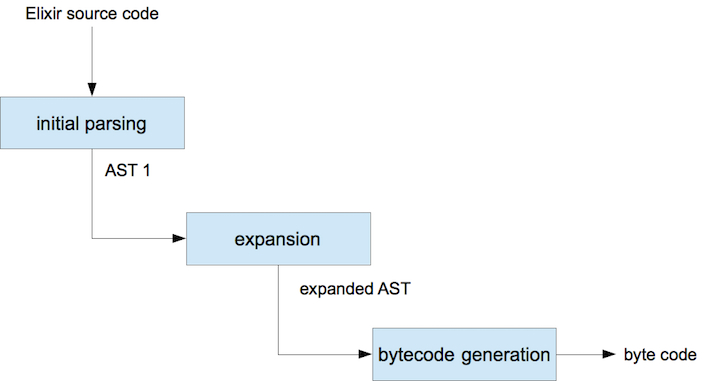
\includegraphics[width=0.6\textwidth]{compilation_process.png}
\end{frame}

\begin{frame}{Metaprogramación en Elixir}{¿Cómo definimos macros?}
  \begin{itemize}
    \item Con el operador \mintinline{elixir}|defmacro| podremos definir
    nuestras macros, respetando las reglas\footnotemark[2]:
    \begin{itemize}
      \item Don't Write macros (WTF?)
      \item Use Macros Gratuitously
    \end{itemize}
    \item El operador \textbf{tiene que} devolver un AST
  \end{itemize}
  \footnotetext[2]{Metaprogramming Elixir: Macro Rules}
\end{frame}

\begin{frame}[fragile]{Definición de macros}{Ejemplo básico}
  \begin{minted}{elixir}
    defmodule ControlFlow do
      defmacro unless(expression, do: block) do
        quote do
          if !unquote(expression), do: unquote(block)
        end
      end
    end
  \end{minted}
\end{frame}

\begin{frame}[fragile]{DEMO}{Un DSL para definir mascotas}
  \begin{columns}
    \begin{column}{0.5\textwidth}
      \scriptsize\begin{minted}{elixir}
        defmodule Template do
          use Pets

          pet "Bucky" do
            species :dog
            hobbies ["sniffing", "eating birds"]
          end
          pet "Gardfield" do
            species :cat
            hobbies ["hating mondays"]
          end
        end
      \end{minted}
    \end{column}
    \begin{column}{0.5\textwidth}
      \scriptsize\begin{minted}{elixir}
        iex> Bucky.greet
        "Hello my name is Bucky and I'm a dog"
        iex> Gardfield.hobbies
        "Gardfield's hobbie is hating mondays"
      \end{minted}
    \end{column}
  \end{columns}
\end{frame}

\begin{frame}{Antipatrones}
  Sobreutilizar esta técnica podría llevarnos a algunos de estos casos\footnotemark[3]:
  \begin{itemize}
    \item \textit{Large code generation}: Cuando la macro genera demasiado código
    \item \textit{Unnecessary macros}: ¿Estás seguro que este código debe ser una macro?
    \item \texttt{use} instead of \texttt{import}: Propagación de dependencias
  \end{itemize}
  \footnotetext[3]{\url{https://hexdocs.pm/elixir/macro-anti-patterns.html}\ (\mintinline{elixir}|>=1.16|)}
\end{frame}

\section{Mi TFM: \texttt{LogicElixir}}
\begin{frame}{Mi TFM: \texttt{LogicElixir}}{Motivación}
  \begin{itemize}
    \item La mayor de todas: aprender sobre metaprogramación (en Elixir).
    \item Hacer mi primer proyecto (serio) en Elixir.
    \item Acabar el Máster :D
  \end{itemize}
\end{frame}

\begin{frame}{\texttt{LogicElixir}}{Objetivo principal}
  \begin{itemize}
    \item Desarrollar una librería para Elixir que permita
    a un programador especificar un programa lógico
    \item Proporcionar mecanismos para realizar consultas sobre
    ese programa lógico
  \end{itemize}
\end{frame}

\begin{frame}[fragile]{\texttt{LogicElixir}: Prerrequisitos}{Programación Lógica}
  \begin{minted}{prolog}
    % Hechos
    human(fry).
    mutant(leela).
    likes(fry, pizza).

    % Reglas
    pizza_lover(X):- likes(X, pizza).

    member(X, [X | _]).
    member(X, [_ | T]):- member(X, T).

  \end{minted}
\end{frame}

\begin{frame}[fragile]{\texttt{LogicElixir}}{Ejemplo}
  \small \begin{minted}{elixir}
    defmodule LogicModule do
      use LogicElixir
      defpred human(:fry)
      defpred mutant(:leela)
      defpred likes(:fry, :pizza)
      defpred pizza_lover(X), do: likes(X, :pizza)
      defpred member(X, [X | T])
      defpred member(X, [H | T]) do
        member(X, T)
      end
    end
  \end{minted}
\end{frame}

\begin{frame}{\texttt{LogicElixir}}{Sintaxis}
  \footnotesize \begin{block}{Términos lógicos}
    \begin{bnfgrammar}
      $T$ ::= $lit$ : literales
        | $X$ : variables lógicas
        | [\,]
        | [$T_1$ \textbar\ $T_2$]
        | \{$T_1$, $T_2$, ..., $T_n$\}
        | $f$($T_1$, $T_2$, ..., $T_n$) : llamadas a funciones de Elixir
    \end{bnfgrammar}
  \end{block}
\end{frame}

\begin{frame}{\texttt{LogicElixir}}{Sintaxis}
  \begin{block}{Patrones}
    \begin{bnfgrammar}
      $P$ ::= $lit$
      | $X$ : variables lógicas
      | [\,]
      | [$P_1$ \textbar\ $P_2$]
      | \{$P_1$, $P_2$, ..., $P_n$\}
    \end{bnfgrammar}
  \end{block}
\end{frame}

\begin{frame}{\texttt{LogicElixir}}{Sintaxis}
  \footnotesize \begin{block}{Objetivos y secuencias de objetivos}
    \begin{bnfgrammar}
      $G$ ::= $\epsilon$ | $g, G$
    ;;
      $g$ ::= $p$($T_1$, $T_2$, ..., $T_n$) : predicados lógicos
          | $T_1$ = $T_2$ : unificación de términos
          | $G_1$ ; ... ; $G_n$ : disyunción de secuencias
          | $@$($e$) : expresiones de Elixir
    \end{bnfgrammar}
  \end{block}
\end{frame}

\begin{frame}{\texttt{LogicElixir}}{Sintaxis}
  \begin{block}{Reglas}
    \begin{equation*}
      R ::= p(P_1, ..., P_n)\,[\,:-\, G]
    \end{equation*}
  \end{block}
  \begin{block}{Definiciones de predicados}
    \begin{equation*}
      D =
      \begin{bmatrix}
        \quad p(P_{1,1},\, \ldots,\, P_{1,n}) \quad [:- \quad G_1]\\
        \quad p(P_{2,1},\, \ldots,\, P_{2,n}) \quad [:- \quad G_2]\\
        \vdots \\
        \quad p(P_{m,1},\, \ldots,\, P_{m,n}) \quad [:- \quad G_m]
      \end{bmatrix}
    \end{equation*}
  \end{block}
\end{frame}

% \subsection{Lenguaje Core}
\begin{frame}{Lenguaje Core}
  \begin{itemize}
    \item El lenguaje Core es el lenguaje de bajo nivel que servirá de nexo
    entre \texttt{LogicElixir} y Elixir.
    \item Una función Core agrupa todos los hechos y reglas de un predicado
    \texttt{defpred} en una única función \texttt{defcore}.
    \item Posee una sintaxis parecida a \texttt{LogicElixir}, pero con matices:
    \begin{itemize}
      \item No existen los patrones.
      \item Ausencia de sintaxis azucarada en las listas.
      \item Los predicados tienen que tener un cuerpo de función.
    \end{itemize}
  \end{itemize}
\end{frame}

% \subsection{Traducción}
\begin{frame}{Traducción de \texttt{LogicElixir} a Core}
  Se considera una definición de predicado $D$:
  \begin{equation*}
    D =
    \begin{bmatrix}
      \quad p(P_{1,1},\, \ldots,\, P_{1,n}) \quad :- \quad G_1\\
      \quad p(P_{2,1},\, \ldots,\, P_{2,n}) \quad :- \quad G_2\\
      \vdots \\
      \quad p(P_{m,1},\, \ldots,\, P_{m,n}) \quad :- \quad G_m
    \end{bmatrix}
  \end{equation*}
\end{frame}

\begin{frame}{Traducción de \texttt{LogicElixir} a Core}
  \begin{columns}
    \column{0.7\textwidth}
    \begin{align*}
      \footnotesize generate\_defcore(D) = \left[
        \begin{array}{lcr}
          \textcolor{blue}{\texttt{defcore}\ } p(X_1, \ldots, X_n) \textcolor{blue}{\ \texttt{do}} \\
          \ \ \ \ \textcolor{blue}{\texttt{choice do}} \\
          \ \ \ \ \ \ \ \ P_{1,1} = X_1 \\
          \ \ \ \ \ \ \ \ \ldots \\
          \ \ \ \ \ \ \ \ P_{1,n} = X_n \\
          \ \ \ \ \ \ \ \ G_1\\
          \ \ \ \ \textcolor{blue}{\texttt{else}} \\
          \ \ \ \ \ldots \\
          \ \ \ \ \textcolor{blue}{\texttt{else}} \\
          \ \ \ \ \ \ \ \ P_{m,1} = X_1 \\
          \ \ \ \ \ \ \ \ \ldots \\
          \ \ \ \ \ \ \ \ P_{m,n} = X_n \\
          \ \ \ \ \ \ \ \ G_m\\
          \ \ \ \ \textcolor{blue}{\texttt{end}} \\
          \textcolor{blue}{\texttt{end}}
        \end{array}
      \right]
    \end{align*}
  \end{columns}
\end{frame}

\begin{frame}[fragile]{Traducción de \texttt{LogicElixir} a Core}{Ejemplos}
  \begin{multicols}{2}
    \footnotesize \begin{minted}{elixir}
      defpred planet(:tatooine)
      defpred planet(:hoth)
      defpred planet(:dagobah)
    \end{minted}
    \columnbreak
    \footnotesize \begin{minted}{elixir}
      defcore planet(X1) do
        choice do
          :tatooine = X1
        else
          :hoth = X1
        else
          :dagobah = X1
        end
      end
    \end{minted}
  \end{multicols}
\end{frame}

\begin{frame}[fragile]{Traducción de \texttt{LogicElixir} a Core}{Ejemplos}
  \begin{multicols}{2}
    \footnotesize \begin{minted}{elixir}
      defpred member(X, [X | T])
      defpred member(X, [H | T]) do
        member(X, T)
      end
    \end{minted}
    \columnbreak
    \footnotesize \begin{minted}{elixir}
      defcore member(X1, X2) do
        choice do
          X = X1
          [X | T] = X2
        else
          X = X1
          [H | T] = X2
          member(X, T)
        end
      end
    \end{minted}
  \end{multicols}
\end{frame}

\begin{frame}[fragile]{Implementación}{\texttt{logic\_elixir.ex}}
  \begin{block}{¿Qué supone la expresión \texttt{use LogicElixir}?}
    Se inyecta un AST a través de la función \texttt{\_\_using\_\_/1}:
    \small\begin{minted}[highlightlines={4}]{elixir}
      defmodule LogicElixir do
        defmacro __using__(_params) do
          quote do
            use LogicElixir.Defpred
            use LogicElixir.Findall
          end
        end
      end
    \end{minted}
  \end{block}
\end{frame}

\begin{frame}[fragile]{Implementación}{\texttt{logic\_elixir.ex}}
  \begin{block}{¿Qué supone la expresión \texttt{use LogicElixir}?}
    Se inyecta un AST a través de la función \texttt{\_\_using\_\_/1}:
    \small\begin{minted}[highlightlines={4}]{elixir}
      defmodule LogicElixir do
        defmacro __using__(_params) do
          quote do
            use LogicElixir.Defpred # <= Dependency injection
            use LogicElixir.Findall
          end
        end
      end
    \end{minted}
  \end{block}
\end{frame}

\begin{frame}[fragile]{Implementación}{\texttt{defpred.ex}}
  \footnotesize \begin{minted}{elixir}
    defmodule LogicElixir.Defpred do
      defmacro defpred(head) do
        {pred_name, args_ast} = Macro.decompose_call(head)
        Module.put_attribute(__CALLER__.module, :definitions,
                              {pred_name, args_ast})
      end

      defmacro defpred(head, do: block) do
        {pred_name, args_ast} = Macro.decompose_call(head)
        Module.put_attribute(__CALLER__.module, :definitions,
                              {pred_name, {args_ast, block}})
      end
    end
  \end{minted}
\end{frame}

\begin{frame}[fragile]{Implementación}{\texttt{defpred.ex}}
  \footnotesize \begin{minted}{elixir}
    defmacro __before_compile__(env) do
      VarBuilder.start_link()
      definitions = Module.get_attribute(env.module, :definitions)
                    |>
                    Enum.reverse()
      grouped_defs = definitions |>
                     Enum.group_by(&elem(&1, 0), &elem(&1, 1))
      for {name, args} <- grouped_defs do
        generate_defcore(name, args)
      end
    end
  \end{minted}
\end{frame}

\begin{frame}{Traducción de Core a función de Elixir}
  \begin{itemize}
    \item El paso final es convertir la definición Core intermedia a código de Elixir.
    \item Para ello, es necesario definir una serie de conjuntos, así como una
    gramática BNF de estos términos disponibles \underline{en tiempo de ejecución}.
  \end{itemize}
\end{frame}

\begin{frame}{Traducción de Core a función de Elixir}{Predicado Core a función Elixir}
  \scriptsize \begin{align*}
    tr\_def(p(X_1, \ldots, X_n)\mathit{:-} G) & = \left[
      \begin{array}{lrl}
        \textcolor{blue}{\texttt{def}}\,\, p(t_1, \ldots, t_n)\,\, \textcolor{blue}{\texttt{do}} \\
          \ \ \ \ x_1 = \textcolor{blue}{\texttt{VarBuilder.gen\_var()}} \\
          \ \ \ \ \vdots \\
          \ \ \ \ x_n = \textcolor{blue}{\texttt{VarBuilder.gen\_var()}} \\
          \ \ \ \ y_1 = \textcolor{blue}{\texttt{VarBuilder.gen\_var()}} \\
          \ \ \ \ \vdots \\
          \ \ \ \ y_m = \textcolor{blue}{\texttt{VarBuilder.gen\_var()}} \\
          \ \ \ \ \textcolor{blue}{\texttt{fn}}\,\, th_1 \textcolor{blue}{\rightarrow} \\
          \ \ \ \ \ \ \ \ th_2 = \textcolor{blue}{\texttt{Map.merge}}(th_1, \\
          \ \ \ \ \ \ \ \ \ \ \ \ \ \ \ \ \textcolor{blue}{\texttt{Map.new}}([\{x_1, t_1\}, \ldots, \{x_n, t_n\}])) \\
          \ \ \ \ \ \ \ \ (tr\_goals(\Delta, G)).(th_2) \\
          \ \ \ \ \ \ \ \ \ \ \ \ \textcolor{blue}{\texttt{|>}} \\
          \ \ \ \ \ \ \ \ \ \ \ \ \textcolor{blue}{\texttt{Stream.map}}(\textcolor{blue}{\&\texttt{Map.drop}(\&1, [}\\
          \ \ \ \ \ \ \ \ \ \ \ \ \ \ \ \ x_1, \ldots, x_n, y_1, \ldots, y_m\textcolor{blue}{]))}\\
          \ \ \ \ \textcolor{blue}{\texttt{end}} \\
          \textcolor{blue}{\texttt{end}}
      \end{array}
    \right]
  \end{align*}
\end{frame}

% \subsection{\texttt{Findall}}
\begin{frame}{Consulta de predicados}
  \begin{itemize}
    \item \texttt{LogicElixir} ofrece un mecanismo de consulta sobre los
    predicados que haya declarado el usuario en su proyecto.
    \item La macro \texttt{findall} sirve de interfaz entre \texttt{LogicElixir}
    y Elixir.
  \end{itemize}
\end{frame}

\begin{frame}{Consulta de predicados}{Lenguaje}
  \begin{equation*}
    F ::= \texttt{findall}\ T\ [\texttt{into}\ E\ ]\ \texttt{do}\ G
  \end{equation*}
  Donde:
  \begin{itemize}
    \item $T$ es un término \texttt{LogicElixir}.
    \item $G$ es una secuencia de objetivos \texttt{LogicElixir}.
    \item $E$ es un término opcional que implementa el protocolo \texttt{Enumerable}.
  \end{itemize}
\end{frame}

\begin{frame}
  \centering
  \huge
  DEMO\\
  \large
  (Probando mi TFM)
\end{frame}

\begin{frame}{Dificultades encontradas}
  \begin{itemize}
    \item Falta de (buena) documentación
    \item Falta de código de apoyo (o desactualizado)
    \item Contramedidas: test unitarios
  \end{itemize}
\end{frame}

\begin{frame}{Conclusiones}
  \begin{itemize}
    \item La metaprogramación es una área bonita (y MUY compleja)
    \item Seguramente nunca tengas que usar esta técnica
    \item No está de más conocer qué hace la ``magia''
    \item Los tests son tus amigos
  \end{itemize}
\end{frame}

\begin{frame}{Bibliografía}
  \begin{thebibliography}{99} % Beamer does not support BibTeX so references must be nserted manually as below
    \bibitem[McCord, 2015]{p1} Chris McCord (2015)
    \newblock Metaprogramming Elixir
  \end{thebibliography}
  \begin{thebibliography}{99} % Beamer does not support BibTeX so references must be nserted manually as below
    \bibitem[Valim, 2023]{p2} José Valim
    \newblock Kernel.SpecialForms, Macro, Module
  \end{thebibliography}
  \begin{thebibliography}{99}
    \bibitem[Sterling \& Shapiro, 1986]{p4} Leon Sterling and Ehud Shapiro (1986)
    \newblock The Art of Prolog
  \end{thebibliography}
  \begin{thebibliography}{99}
    \bibitem{LogicElixir} \url{https://github.com/MiguelERuiz/logic\_elixir}
    \newblock Repo de la librería \texttt{LogicElixir}
  \end{thebibliography}
  \begin{thebibliography}{99}
    \bibitem{LogicElixirExamples} \url{https://github.com/MiguelERuiz/logic\_elixir\_examples}
    \newblock Repo de uso de la librería \texttt{LogicElixir}
  \end{thebibliography}
\end{frame}

\begin{frame}{Otros recursos}
  \begin{thebibliography}{99}
      \bibitem{ChrisMcCord} \url{https://chrismccord.com/blog/2014/03/13/write-less-do-more-and-have-fun-with-elixir-macros/}
      \newblock Charla de Chris McCord en la ElixirConf (2014)
  \end{thebibliography}
  \begin{thebibliography}{99}
      \bibitem{SasaJuric} \url{https://www.theerlangelist.com/article/macros_1}
      \newblock Blog de Sasa Juric sobre Macros (2014)
  \end{thebibliography}
  \begin{thebibliography}{99}
      \bibitem{RepoPets} \url{https://github.com/MiguelERuiz/pets}
      \newblock Repo de Pets
  \end{thebibliography}
  \begin{thebibliography}{99}
      \bibitem{RepoSlides} \url{https://github.com/MiguelERuiz/presentations}
      \newblock Repo de Presentaciones
  \end{thebibliography}
\end{frame}
\end{document}